\documentclass{article}

% packages
  % basic stuff for rendering math
  \usepackage[letterpaper, top=1in, bottom=1in, left=1in, right=1in]{geometry}
  \usepackage[utf8]{inputenc}
  \usepackage[english]{babel}
  \usepackage{amsmath} 
  \usepackage{amssymb}
  \usepackage{amsthm}

  % extra math symbols and utilities
  \usepackage{mathtools}        % for extra stuff like \coloneqq
  \usepackage{mathrsfs}         % for extra stuff like \mathsrc{}
  \usepackage{centernot}        % for the centernot arrow 
  \usepackage{bm}               % for better boldsymbol/mathbf 
  \usepackage{enumitem}         % better control over enumerate, itemize
  \usepackage{hyperref}         % for hypertext linking
  \usepackage{fancyvrb}          % for better verbatim environments
  \usepackage{newverbs}         % for texttt{}
  \usepackage{xcolor}           % for colored text 
  \usepackage{listings}         % to include code
  \usepackage{lstautogobble}    % helper package for code
  \usepackage{parcolumns}       % for side by side columns for two column code
  

  % page layout
  \usepackage{fancyhdr}         % for headers and footers 
  \usepackage{lastpage}         % to include last page number in footer 
  \usepackage{parskip}          % for no indentation and space between paragraphs    
  \usepackage[T1]{fontenc}      % to include \textbackslash
  \usepackage{footnote}
  \usepackage{etoolbox}

  % for custom environments
  \usepackage{tcolorbox}        % for better colored boxes in custom environments
  \tcbuselibrary{breakable}     % to allow tcolorboxes to break across pages

  % figures
  \usepackage{pgfplots}
  \pgfplotsset{compat=1.18}
  \usepackage{float}            % for [H] figure placement
  \usepackage{tikz}
  \usepackage{tikz-cd}
  \usepackage{circuitikz}
  \usetikzlibrary{arrows}
  \usetikzlibrary{positioning}
  \usetikzlibrary{calc}
  \usepackage{graphicx}
  \usepackage{algorithmic}
  \usepackage{caption} 
  \usepackage{subcaption}
  \captionsetup{font=small}

  % for tabular stuff 
  \usepackage{dcolumn}

  \usepackage[nottoc]{tocbibind}
  \pdfsuppresswarningpagegroup=1
  \hfuzz=5.002pt                % ignore overfull hbox badness warnings below this limit

% New and replaced operators
  \DeclareMathOperator{\Tr}{Tr}
  \DeclareMathOperator{\Sym}{Sym}
  \DeclareMathOperator{\Span}{span}
  \DeclareMathOperator{\std}{std}
  \DeclareMathOperator{\Cov}{Cov}
  \DeclareMathOperator{\Var}{Var}
  \DeclareMathOperator{\Corr}{Corr}
  \DeclareMathOperator{\pos}{pos}
  \DeclareMathOperator*{\argmin}{\arg\!\min}
  \DeclareMathOperator*{\argmax}{\arg\!\max}
  \newcommand{\ket}[1]{\ensuremath{\left|#1\right\rangle}}
  \newcommand{\bra}[1]{\ensuremath{\left\langle#1\right|}}
  \newcommand{\braket}[2]{\langle #1 | #2 \rangle}

% Custom Environments
  \newtcolorbox[auto counter, number within=section]{theorem}[1][]
  {
    colframe = red!25,
    colback  = red!10,
    coltitle = red!20!black,  
    breakable, 
    title = \textbf{Theorem \thetcbcounter ~(#1)}
  } 
  \newtcolorbox[auto counter, number within=section]{proposition}[1][]
  {
    colframe = red!25,
    colback  = red!10,
    coltitle = red!20!black,  
    breakable, 
    title = \textbf{Proposition \thetcbcounter ~(#1)}
  } 
  \newtcolorbox[auto counter, number within=section]{corollary}[1][]
  {
    colframe = red!25,
    colback  = red!10,
    coltitle = red!20!black,  
    breakable, 
    title = \textbf{Corollary \thetcbcounter ~(#1)}
  } 
  \newtcolorbox[auto counter, number within=section]{definition}[1][]
  {
    colframe = yellow!25,
    colback  = yellow!10,
    coltitle = yellow!20!black,  
    breakable, 
    title = \textbf{Definition \thetcbcounter ~(#1)}
  } 
  \newtcolorbox[auto counter, number within=section]{example}[1][]
  {
    colframe = blue!25,
    colback  = blue!10,
    coltitle = blue!20!black,  
    breakable, 
    title = \textbf{Example \thetcbcounter ~(#1)}
  } 
  \newtcolorbox[auto counter, number within=section]{code}[1][]
  {
    colframe = green!25,
    colback  = green!10,
    coltitle = green!20!black,  
    breakable, 
    title = \textbf{Code \thetcbcounter ~(#1)}
  } 
  \newtcolorbox[auto counter, number within=section]{algo}[1][]
  {
    colframe = green!25,
    colback  = green!10,
    coltitle = green!20!black,  
    breakable, 
    title = \textbf{Algorithm \thetcbcounter ~(#1)}
  } 

  \BeforeBeginEnvironment{example}{\savenotes}
  \AfterEndEnvironment{example}{\spewnotes}
  \BeforeBeginEnvironment{lemma}{\savenotes}
  \AfterEndEnvironment{lemma}{\spewnotes}
  \BeforeBeginEnvironment{definition}{\savenotes}
  \AfterEndEnvironment{definition}{\spewnotes}
  \BeforeBeginEnvironment{corollary}{\savenotes}
  \AfterEndEnvironment{corollary}{\spewnotes}
  \BeforeBeginEnvironment{proposition}{\savenotes}
  \AfterEndEnvironment{proposition}{\spewnotes}
  \BeforeBeginEnvironment{theorem}{\savenotes}
  \AfterEndEnvironment{theorem}{\spewnotes}
  \BeforeBeginEnvironment{exercise}{\savenotes}
  \AfterEndEnvironment{exercise}{\spewnotes}
  \BeforeBeginEnvironment{solution}{\savenotes}
  \AfterEndEnvironment{solution}{\spewnotes}
  \BeforeBeginEnvironment{question}{\savenotes}
  \AfterEndEnvironment{question}{\spewnotes}
  \BeforeBeginEnvironment{code}{\savenotes}
  \AfterEndEnvironment{code}{\spewnotes}
  \BeforeBeginEnvironment{algo}{\savenotes}
  \AfterEndEnvironment{algo}{\spewnotes}

  \definecolor{dkgreen}{rgb}{0,0.6,0}
  \definecolor{gray}{rgb}{0.5,0.5,0.5}
  \definecolor{mauve}{rgb}{0.58,0,0.82}
  \definecolor{darkblue}{rgb}{0,0,139}
  \definecolor{lightgray}{gray}{0.93}
  \renewcommand{\algorithmiccomment}[1]{\hfill$\triangleright$\textcolor{blue}{#1}}

  % default options for listings (for code)
  \lstset{
    autogobble,
    frame=ltbr,
    language=Python,
    aboveskip=3mm,
    belowskip=3mm,
    showstringspaces=false,
    columns=fullflexible,
    keepspaces=true,
    basicstyle={\small\ttfamily},
    numbers=left,
    firstnumber=1,                        % start line number at 1
    numberstyle=\tiny\color{gray},
    keywordstyle=\color{blue},
    commentstyle=\color{dkgreen},
    stringstyle=\color{mauve},
    backgroundcolor=\color{lightgray}, 
    breaklines=true,                      % break lines
    breakatwhitespace=true,
    tabsize=3, 
    xleftmargin=2em, 
    framexleftmargin=1.5em, 
    stepnumber=1
  }

% Page style
  \pagestyle{fancy}
  \fancyhead[L]{Development Tools}
  \fancyhead[C]{Muchang Bahng}
  \fancyhead[R]{Fall 2024} 
  \fancyfoot[C]{\thepage / \pageref{LastPage}}
  \renewcommand{\footrulewidth}{0.4pt}          % the footer line should be 0.4pt wide
  \renewcommand{\thispagestyle}[1]{}  % needed to include headers in title page

\begin{document}

\title{Development Tools}
\author{Muchang Bahng}
\date{Fall 2024}

\maketitle
\tableofcontents
\pagebreak

\section{Neovim} 

  The first thing you do when coding is typing something, and this requires a text editor. 

\section{Git} 

    Git is a pretty complex version control tool. It allows you to perform different actions. We'll go over them, starting with the most basic to the most complex. In order to learn this, we should know the structure of the git history. 

  \subsection{Local Git Repository} 

    When you do \texttt{git init} in a repository, you are essentially saying that you want to keep track of the history of this repository. This can obviously be done with an undo tree, which comes out-of-box in almost all text editors, but it is much more powerful. 

    \begin{definition}[Local Git Tree]
      The history of our repository is essentially a tree, with each node representing some edits composed of 
      \begin{enumerate}
        \item adding a new file 
        \item modifying a file 
        \item deleting a file
      \end{enumerate} 
      Each node is represented by a hash generated from its previous node and the corresponding edits. You can see your history using  
      \begin{lstlisting}
        git log 
      \end{lstlisting} 
      \texttt{HEAD} is a pointer to the node that reflects the state of your current repository (minus your uncommitted edits), which is usually the most recent node. 
    \end{definition} 

    Unlike most undo trees, these nodes are not added automatically. You must add them manually through a 2-step process. 

    \begin{definition}[Stage]
      You want to take a set of edits and \textbf{stage} them. This essentially tells git that these staged files/lines are going to be a part of the next node. 
    \end{definition}

    \begin{definition}[Commit]
      Then you commit your changes, which does the following. 
      \begin{enumerate}
        \item This takes all of your staged changes and packages them in a node $A$. 
        \item It looks at \texttt{HEAD}, uses \texttt{HEAD}'s hash to generate the hash of $A$, and appends $A$ to \texttt{HEAD} by having $A$ point to \texttt{HEAD}.\footnote{So nodes actually point to \textit{previous nodes}.}
        \item It moves \texttt{HEAD} to $A$. 
      \end{enumerate}
    \end{definition} 

    Therefore, when you make your first commit, you are creating a genesis node from which every other edit will be based off of. Your \texttt{HEAD} then points to this commit. This is great start, and let's add more functionality. 

    \begin{definition}[Checkout a Commit]
      You can move \texttt{HEAD} to point to a specific commit by using 
      \begin{lstlisting}
        git checkout <commit-hash>  # point to this commit  
        git checkout HEAD~N         # point to the commit $N$ nodes before HEAD
      \end{lstlisting} 
      This leaves you in a \texttt{detached head state}, which means that your head is not pointing to the end node. This is useful if you want to 
      \begin{enumerate}
        \item \textit{explore the codebase at a commit's snapshot in time}. 
      \end{enumerate}
    \end{definition} 

    Note that so far, we have described git as a linked list plus some extra head pointer. Adding to this linked list is easy since we are simply adding new edits, but deleting can be very tricky. We will first introduce how to delete the most recent $K$ commits, which is the easiest way to delete. 

    \begin{definition}[Reset] 
      Say that your history is 
      \begin{equation}
        (A) \leftarrow (B) \leftarrow (C) \leftarrow (H \mapsto D)
      \end{equation}  
      If we want to throw away commits $C$ and $D$, we can \textbf{reset} to $B$, which deletes $C, D$ and has $H$ point to $B$, giving us 
      \begin{equation}
        (A) \leftarrow (H \mapsto B)
      \end{equation} 
      \begin{enumerate}
        \item A \textbf{soft reset} means that the edits introduced in $C$ and $D$ will still be kept as unstaged changes, and so you may use them as a starting point to make your next commit. 
        \item A \textbf{hard reset} means that the edits are also completely deleted. 
      \end{enumerate}
    \end{definition} 

    Most beginners in git really know these commands when working with their history, but this is really just a glorified stack. The additional operations can be daunting because they have the risk of introducing \textit{conflicts}. 

  \subsection{Conflicts} 

    \begin{definition}[Conflicts]
      A \textbf{conflict} arises when two commits contain edits that change some location independently at the same time. They occur most frequently when working with multiple branches, but they can happen even when working on a single branch. Git will tell you when there is conflict between commits $C$ and $C^\prime$ at a certain location. At this point, you will have to manually go to that location and compare the changes introduced in $C$ and $C^\prime$, called \textbf{hunks}. The conflict looks generally like this. 
      \begin{lstlisting}
        ... some code above 
        <<<<< (C)   # hunk 1
        ========
        >>>>> (C')  # hunk 2
        ... some code below
      \end{lstlisting} 

      In order to fix this conflict, you can  
      \begin{enumerate}
        \item select hunk 1 (and ignore hunk 2)
        \item select hunk 2 
        \item select both hunks (i.e. incorporate both edits) 
        \item manually delete the \texttt{>>>}, \texttt{===}, \texttt{<<<} and directly edit the file to make a custom change that overrides both hunks. 
      \end{enumerate} 
    \end{definition} 

    Choosing the option to fix a conflict may sometimes be complicated, since you may not always want to select the hunk reflected in your most recent changes, because doing that might introduce another conflict in a later commit that actually modified the old code into the new code. 

    \begin{definition}[Revert Commit] 
      Say that you have history
      \begin{equation}
        (C_1) \leftarrow (C_2) \leftarrow (C_3) \leftarrow (H \mapsto C_4)
      \end{equation} 
      You can choose to \textbf{revert} and of the 4 commits above. Given any commit $C$, reverting a commit means that you simply add a new commit $C^\prime$ with the changes that are the exact opposite of $C$. If we want to revert commit $C_2$, our history looks like 
      \begin{equation}
        (C_1) \leftarrow (C_2) \leftarrow (C_3) \leftarrow (C_4) \leftarrow (C_2^\prime)
      \end{equation}  
      So really, we are ``deleting'' our history by adding. 
    \end{definition} 

    \begin{example}[Conflicts in Reverting]
      Say that you have history
      \begin{equation}
        (C_1) \leftarrow (C_2) \leftarrow (C_3) \leftarrow (H \mapsto C_4)
      \end{equation} 
      If you try to revert $H$, this is fine and will never have conflicts. Say that you made an edit in $(C_3)$ where you added $x = 4$ to some python script, and then you removed this line in $(C_4)$. Then if you add $(C_3^\prime)$ to undo it, it tries to delete a line that isn't even there! Therefore you will get a conflict that looks something like 
      \begin{lstlisting}
        <<<<< (C4)   # hunk 1 
        - x = 4 
        ========
        - x = 4
        >>>>> (C3')  # hunk 2
      \end{lstlisting}
      Obviously you can just select either one of the hunks to get what you want. 
    \end{example} 

    Conflicts are unavoidable and you will have to get comfortable with them.  

  \subsection{Interactive Rebasing} 

    Even though we can revert commits, we haven't actually found out how to truly \textit{delete} a commit from your history which modifies 
    \begin{equation}
      (A) \leftarrow (B) \leftarrow (C) \leftarrow (D)
    \end{equation} 
    to something like 
    \begin{equation}
      (A) \leftarrow (B) \leftarrow (D)
    \end{equation} 
  
    \begin{definition}[Rebasing]
      Essentially, we want to \textit{directly} (unlike a revert) modify our history that goes \textit{beyond} (unlike a reset) the last $K$ commits. Any actions that modifies the history is known as \textbf{rebasing}, which can be done automatically by git but must often be done \textbf{interactively}. When you want to start an interactive rebase, you want to tell git from which commit $C_s$ you want to start the interactive rebase on. 
      \begin{lstlisting}
        git rebase -i <start commit hash>
      \end{lstlisting}
      You are saying that from commit $C_s$ and beyond until the end $C_n$, I may arbitrarily modify them, but commits previous to $C_s$ will be untouched. When you do this, all commits $C_i$ where $i \geq s$ will be shown as below. 

      \begin{figure}[H]
        \centering 
        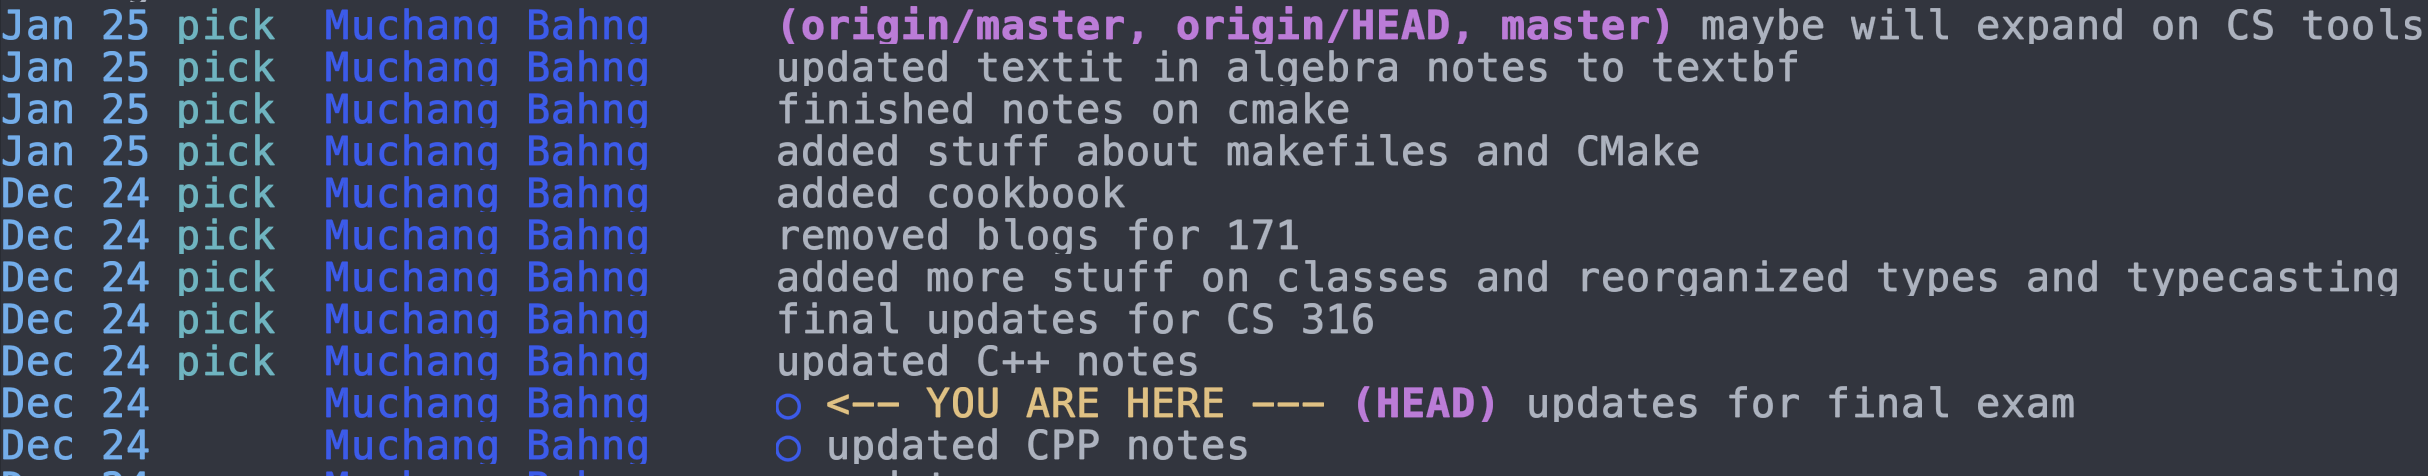
\includegraphics[scale=0.3]{img/rebase.png}
        \caption{Interactive rebase shown in LazyGit.} 
        \label{fig:rebase}
      \end{figure}

      There are a fixed set of supported operations allows in an interactive rebase.\footnote{Note that pick and reword will never cause conflicts. Squash and fixup will most likely not cause conflicts. Drop, break, edit, and swapping may cause conflicts.}
      \begin{enumerate}
        \item \textbf{Pick}. This just means that you are leaving the commit alone, i.e. picking it to be in the rebase. 
        \item \textbf{Reword}. Just edits the commit message. 
        \item \textbf{Squash}. Given commit $C_i \leftarrow C_{i+1}$, you can label $C_{i+1}$ with \texttt{squash} to merge it into $C_{i}$, turning 2 nodes into one. This almost never causes conflicts. The new commit message is just those of $C_{i}, C_{i+1}$ concatenated. 
        \item \textbf{Fixup}. Like squash, but discard the commit's message.  
        \item \textbf{Drop}. This deletes a commit and removes it entirely.  
        \item \textbf{Break}. Stop at this commit to edit it. I think you can change which edits you have committed, choose which edits to keep, and choose which edits to remove (back into your unstaged changes). 
        \item \textbf{Edit}. Stop at this commit to amend it. 
        \item You can also swap commits by editing the text file so that the commits are in a different order. 
          \begin{lstlisting}
            # Original order in rebase editor:
            pick abc123 First commit
            pick def456 Second commit

            # After swapping lines in editor:
            pick def456 Second commit
            pick abc123 First commit 
          \end{lstlisting}
      \end{enumerate} 
      After you edit the rebase text file and continue the rebase, git will do the following sequentially: 
      \begin{enumerate}
        \item \texttt{HEAD}, which pointed at $C_n$, will point towards $C_s$. 

        \item While \texttt{HEAD} is pointing at $C_i \neq C_n$ (i.e. not at the end), we do the following. 
          \begin{enumerate}
            \item It will attempt to perform all the operations you have specified for the next commit $C_{i+1}$. 
            \item If the operations are finished, we increment \texttt{HEAD} to point to $C_{i+1}$ and continue. 
            \item If there is a conflict, it will pause, state that there are conflicts between $\texttt{HEAD} = C_i$ and $C_{i+1}$, and ask you to resolve them. Once resolved it will continue. 
          \end{enumerate} 

        \item Then we are done with the rebase since we have went through all commits, modified them, and resolved all conflicts. 
      \end{enumerate}
      Interactive rebasing is an extremely powerful way to modify your commit history, and it's probably the operation where you'll spend the most time on git. 
    \end{definition} 

    Again, note that if you have changed anything in commit $C_i$, then the hash of $C_i$ every $C_j$ after will get changed. This causes git to interpret these changed commits as completely new ones, even if we only picked a given commit without any modifications. For single-branch rebases, this is fine, but this causes some nasty problems when rebasing over multiple branches, as we will talk about later. 

  \subsection{Branches} 

    Okay, so we now have much better control over our git history, but we've only been treating our history as a linked list. In order to introduce the tree structure, we need to introduce the \textit{branch}. This is especially important if we have a particular previous commit $C_{k < n}$ where we would like to make some different changes to, giving us \textbf{diverging histories} with next nodes $C_k \leftarrow C_{k+1}$ and $C_k \leftarrow C_{k^\prime + 1}$. 
    
    \begin{definition}[Branch]
      A \textbf{branch} is a path from the root commit to any leaf node. It represents a unique history from genesis to \texttt{HEAD}. To list all branches, use 
      \begin{lstlisting}
        >> git branch 
          feature/threading
        * main
          test/tensor
      \end{lstlisting} 
      The asterisk represents which branch you are currently on. The first branch you start off with is a special branch called \textbf{main}, or \textbf{master} branch. 
    \end{definition} 

    Therefore, really our linked-list history is a git tree with a single branch. 

    \begin{definition}[Creating/Switching Branches]
      From any (main or non-main) branch you can create new branches by choosing the commit to split from. 
      \begin{enumerate}
        \item Create a new branch from HEAD of current branch. 
          \begin{lstlisting}
            git branch <new-branch-name> 
          \end{lstlisting}

        \item Create a new branch from certain commit of current branch. 
          \begin{lstlisting}
            git branch <new-branch-name> <commit-hash>
          \end{lstlisting} 

        \item To switch to another branch 
          \begin{lstlisting}
            git checkout <branch> 
          \end{lstlisting}
      \end{enumerate}
    \end{definition} 

    \subsubsection{Working Between Branches} 

      If you are simultaneously working on multiple branches, you may have to checkout/switch between branches frequently. Often, you may have uncommitted changes before you checkout, and git does not allow you to do this. Therefore, we can \textit{stash} them. 

      \begin{definition}[Stash]
        \textbf{Stashing} changes mean that you can take uncommitted changes and store them in a temporary node but not have it point to any existing commit in a branch. This allows you to save your changes without having to commit incomplete work to a branch, and you can pop them back whenever you need. 
      \end{definition} 

    \subsubsection{Merge} 

      \begin{definition}[Fast-Forward Merge]
        
      \end{definition}

    \subsubsection{Rebase}

      \begin{definition}[Rebase]
        
      \end{definition}

      \begin{definition}[Rebasing Diamond Merges]
        
      \end{definition}
    
  \subsection{Remote Trees}

    This allows you to keep track of your change history, but another benefit is to store these changes in the cloud. In order to do this, you must have access to a remote server. 

    \begin{definition}[Remote References]
      In your local branch, it 
    \end{definition}

    \begin{definition}[Remote Git Tree]
      
    \end{definition}

    \begin{definition}[Fetch]
      
    \end{definition}

    \begin{definition}[Fast-Forward]
      
    \end{definition}

    \begin{definition}[Push]
      
    \end{definition}

\section{Continuous Integration (CI)} 

  \textbf{Continuous integration (CI)}, or \textbf{continuous development (CD)}, refers to any automated process that runs whenever you perform some action on a repository. These can include: 
  \begin{enumerate}
    \item Compiling your package upon pushing to a git branch. This saves the time of manually compiling it yourself. 
    \item Compiling and/or running unit tests on your package, over possibly different compiler/interpreter versions on different operating systems and different architectures, whenever someone opens a pull request. This is usually done by automatically creating docker images and running a script that sets up the environment for your system. 
    \item Automatically publishing a new package version to PyPI upon a push to the master branch of a repository. 
  \end{enumerate} 

  \textbf{Github actions} provide \textbf{workflow scripts} that you can include in your repository's \texttt{github/workflows/} directory that automates this. They are essentially yaml files that activate upon some command, whether that'd be a push to a branch, a pull request, or even the completion/failure of another workflow. This gives great convenience in deploying code. 

  

\section{}


\end{document}
